\documentclass[12pt]{article}
\usepackage[utf8]{inputenc}
\usepackage{libertine}
\usepackage[varg]{newtxmath}
\usepackage{amsmath}
\usepackage{amsfonts}
\usepackage{amssymb}
\usepackage{hyperref}
\usepackage{graphicx}
\usepackage{natbib}

\def\D{\mathrm{d}}

\newtheorem{remark}{Remark}

\setlength{\parindent}{0ex}
\setlength{\parskip}{1em}%Espacement des par

\newcommand{\E}[1]{\operatorname{E}\left[#1\right]}
\newcommand{\Et}[1]{\operatorname{E}_t\left[#1\right]}
\newcommand{\V}[1]{\operatorname{Var}\left[#1\right]}
\newcommand{\cov}[1]{\operatorname{Cov}\left(#1\right)}
\newcommand{\covt}[1]{\operatorname{Cov}_t\left(#1\right)}
\newcommand{\avg}[2]{\frac{#1}{#2} \sum_{i=#1}^{#2}}
\def\D{\mathrm{d}}
\newcommand{\Prob}[1]{\operatorname{Pr}\left[#1\right]}
\newcommand{\Probhat}[1]{\hat{\operatorname{Pr}}\left[#1\right]}
\newcommand{\plim}{\operatorname{plim}}
\newcommand{\pconv}{\overset{\text{p}}{\to}}
\newcommand{\dconv}{\overset{\text{d}}{\to}}
\newcommand{\msconv}{\overset{\text{ms}}{\to}}
\def\D{\mathrm{d}}


\title{\vspace{-70pt} ECON8855 - Replication Results\\ \textbf{The Costs of Environmental Regulation in a Concentrated Industry} \\ \textit{by Stephen P. Ryan}}
\author{replicated by Paul Anthony Sarkis}

\begin{document}

\maketitle

\section{Context}

The research question that is intended to answer in this paper is whether the Clean Air Act (CAA) had any dynamic effects on the Portland Cement industry in the United States. In fact, the CAA, by enforcing stricter environmental regulations, increased investment costs and sunk costs in most polluting industries. These regulations have always been analyzed using engineering estimates that tend to forget about (1) sunk costs and (2) dynamic effects. By using the Bajari, Benkard and Levin (2007) estimator on a dynamic oligopoly model, the author will try to recover the structural parameters such as entry costs, exit costs and investment costs for both the pre-1990 and post-1990 periods (before and after the CAA). 

In order to understand the paper, one needs to understand what the Bajari, Benkard and Levin (henceforth BBL) procedure is all about. Ideally, one would want to estimate all parameters of the dynamic oligopoly model by solving the game for each guess of parameters. However, this procedure would be computationally costly, and thus would reduce the potential size of the problem to analyze. To go around this issue, BBL provides a two-step estimation procedure. In the first step, they estimate ``policy functions'' which are accurate descriptions of agents' static behavior given the state of the world. Using these policy functions, there is no need to solve the model anymore, we just need to move from state to state using the policy function estimates. To recover the dynamic structural parameters, the second step will try to find the parameters that ``justify'' the estimated policy functions, using private shocks that follow a certain distribution. The estimation of this distribution, and whether it changes from the pre- to the post-1990 periods is the main result of this paper.

In this paper, the Portland Cement Industry is studied. The dynamic oligopoly model consists of firms competing à la Cournot in each period, making investments to their capacity and potentially entering/exiting the market. The state vector of this problem consists of the firms' capacities in a given market. Thus, policy functions will be estimated on all decisions that affect these state variables: investment, entry and exit. The Cournot game is a way to get static per-period profit that will help identifying the structural parameters. Then, the second step will estimate the distributions of shocks as explained above. These shocks are of four kinds in this paper: entry costs, exit costs (scrap value), investment and divestment. The idea is to find the parameters of these distributions that would imply the estimated policy functions.

The rest of this replication is organized as follows: in section 2, I will introduce the datasets shared by the author and replicate summary statistics. Then, in the first half of section 3, I will show the results obtained on the policy function estimation parts and on solving the Cournot model. Finally, in the last half of section 3, I will explain the main challenges in the dynamic estimation that prevented me from getting to replicate these results. Implementation of the empirical strategy is done in Julia and a bit of Python. All codes are available in the associated GitHub repository, available at the following link: \url{https://github.com/sarkispa/EnvRegCement}.

\section{Data and Summary Statistics}

There are two datasets shared (and used) in this paper: the first one combines supply and demand data at the market level, while the second one consists of production and investment data at the plant level. In order to replicate the results, the necessary first step was to compare the summary statistics that could be extracted from the dataset shared and the ones presented in the paper. The summary statistics of this  replication are presented in Table \ref{tab:summstat}.

Already, discrepancies appear in some ``interior'' statistics like the mean and standard deviation. Moreover, the text mentions 27 different markets while a simple grouping of the dataset shared yields only 22 markets. After further investigation, I found two reasons for that. First of all, some markets are supposed to be differentiated and are not in the dataset shared. For example, in the Minerals Yearbook, the state of Pennsylvania is divided between western PA and eastern PA. However, the shared data only shows PA (with two observations per year). I had to come back to the Yearbooks and separate these markets ``by hand''. Since this affected three states (PA, TX and CA), it yielded three more markets. The second reason for the lower number of markets comes from a intrinsic flaw in the shared dataset. In fact, the Minerals Yearbook defines all markets in the industry as half-states (as in the PA case), whole states or combinations of two or more states. This definition is stable over the years so there were no changes throughout the sample used in the paper. Nonetheless, for some reason, some combinations of states do not correspond to the ones in the Yearbook. It is not clear if the author used the true combinations or the ones in the shared dataset, however, from the fact that I am not getting even the summary statistics right, I guess that he shared a reshuffled dataset. This fact needs to be taken into account when trying to interpret the results of this replication.\\

\begin{table}[ht!]
\centering
\begin{tabular}{lrrrr}
\hline \hline
Variable & Min. & Mean & Max. & S.D. \\ \hline
\textbf{Market-level data} & \textbf{} & \textbf{} & \textbf{} & \textbf{} \\
Quantity & 186 & 2850.59 & 10262 & 1575.07 \\
Price & 39.35 & 67.94 & 138.99 & 13.73 \\
Plants in mkt & 1 & 4.77 & 20 & 1.97 \\
Skilled wage & 20.14 & 31.68 & 44.34 & 4.38 \\
Coal price & 15.88 & 26.90 & 42.33 & 8.24 \\
Electricity price & 4.23 & 5.71 & 7.6 & 1.02 \\
Nat. gas price & 3.7 & 6.26 & 24.3 & 2.27 \\
Pop. & 689,584 & 10,029,721 & 331,000,000 & 7,410,532 \\
 &  &  &  &  \\
\textbf{Plant-level data} & \textbf{} & \textbf{} & \textbf{} & \textbf{} \\
Quantity & 158 & 694 & 2348 & 348 \\
Capacity & 0 & 789 & 3118 & 392 \\
 &  &  &  &  \\
\textbf{Firm-level data} & \textbf{} & \textbf{} & \textbf{} & \textbf{} \\
Cap. investment & -1,509 & 33.64 & 2,573 & 251 \\ \hline \hline
\end{tabular}
\caption{Summary statistics}
\label{tab:summstat}
\end{table}


\section{Main Results}

\subsection{Product Market Profits and Policy Functions}

This part of Section 3 is aimed at presenting both the Cournot game estimation and the policy functions estimation.

\subsubsection{Cement Demand}

The estimation of cement demand is pretty straightforward. Using the panel data of production, prices and other market characteristics at the market-year level, a log-log demand specification is estimated. In particular, the regression is defined as: $$\ln Q_{jt} = \alpha_0 + \alpha_1\ln P_{jt} + \alpha_{2j} + \alpha_{3t}'X_{jt} + \epsilon_{jt} $$
Endogeneity of prices is instrumented with supply-shifters such as input costs (gas, coal and electricity) and labor costs (wages). Other controls typically relate to the size of the market's economy using population, number of housing permits, etc. In the end, these covariates do not matter since the author chooses a specification that does not include them. Market-level fixed-effects are nonetheless included in the regression. Results of all specifications are shown in Table \ref{tab:demand}. Specification III is the one chosen by the author.

\begin{table}[ht!]
\centering
\begin{tabular}{lrrrrrr}
\hline \hline
 & I & II & III & IV & V & VI \\ \hline
Price & -2.69 & -1.77 & -1.86 & -0.097 & -1.70 & -0.014 \\
 & (0.302) & (0.258) & (0.264) & (0.157) & (0.310) & (0.129) \\
Intercept & 19.1 & 9.20 &  &  & 8.75 &  \\
 & (1.27) & (1.38) &  &  & (1.60) &  \\
Log pop. &  & 0.38 &  & 0.852 & 0.283 & 0.797 \\
 &  & (0.033) &  & (0.037) & (0.059) & (0.035) \\
Log permits &  &  &  &  & 0.157 & 0.327 \\
 &  &  &  &  & (0.059) & (0.037) \\
Market FE? & No & No & Yes & Yes & No & Yes \\ \hline \hline
\end{tabular}
\caption{Cement Demand Estimates}
\label{tab:demand}
\end{table}

We can see that the results are quite different from the ones presented in the paper. As mentioned in the previous section, we need to take into account the fact that this estimation is done on a different dataset, with different market definitions. It would not be surprising that this fact alone drives the differences in the estimates. In the rest of the replication, I also used specification III (although the parameters are not the same as in the paper).

\subsubsection{Production Costs}

The estimation of production costs is done using nonlinear least-squares on the difference between simulated market quantities and actual quantities. Although the execution can prove to be quite cumbersome, the intuition is quite simple. In fact, having estimated demand for each market, we assume all firms share the same cost function in the form of: $$C(q_i, s_i; \delta) = \delta_1 \cdot q_i + \delta_2 \cdot 1[q_i > \nu\cdot s_i] \cdot (q_i - \nu\cdot s_i)^2 $$
Then, using this cost function, we solve for the Cournot equilibrium quantities in all markets and compare them to actual quantities. Then, the nonlinear least-squares estimation procedure solves for the parameter vector $\delta$ that minimizes the average square distance between simulated and actual quantities. Note that two estimations are done: one for pre-1990 markets and one for post-1990 markets (1990 included). The final results are shown in Table \ref{tab:prodcosts}.

\begin{table}[ht!]
\centering
\begin{tabular}{lrr}
\hline \hline
Parameter & Pre-1990 Coef. & Post-1990 Coef. \\ \hline
Marginal cost ($\delta_1$) & 24.889 & 29.668 \\
Capacity cost ($\delta_2$) & 0.238 & 0.636 \\
Capacity threshold ($\nu$) & 0.809 & 0.900 \\ \hline \hline
\end{tabular}
\caption{Cost Function Estimates}
\label{tab:prodcosts}
\end{table}

We can see that the results that are achieved in this step are mixed. First, we can see that both $\delta_1$ and $\nu$ are somewhat close to the results presented in the paper. However, the estimated value of $\delta_2$ varies widely between the replication and the paper. In order to compare them further, a good test is to evaluate the average least-squares deviation for different values of $\delta_2$ and compare. Even though the differences might come from using different datasets, I show in figures \ref{fig:d2comp}, \ref{fig:d2comp-p90}, \ref{fig:d2comp-r} and \ref{fig:d2comp-p90-r} that the values I estimated for $\delta_2$ are better than Ryan's estimates, regardless of the values of other parameters. Again, I cannot stress enough that this is not putting the author's work in question but rather showing that given my model and data, the parameters I find are actually the optimal parameters.

To finish this section, I will explain my strategies to solve the nonlinear least-squares procedure. First of all, a Cournot model needs to be solved. In this simple Nash-in-quantities game, I solve for the equilibrium quantities for each market at each period of time, given a demand function estimate (fixed) and a ``guess'' of the cost function parameters. Solving the model is done using the Mixed Complementarity Problem framework and the PATH Solver implementation in Julia. I then proceed to store these simulated quantities in a vector and compare them to the actual quantities vector using a mean-square error metric. From the definition of this problem it seems obvious that the objective function (the MSE) is highly nonlinear, taking different values for each vector of parameters. This is due to the fact that three parameters have to explain supply-side behavior of all firms in all markets for all years within each period (pre-and-post-1990). Changing the value of one parameter might make the prediction of equilibrium quantity of a firm better but then worsen the predictions in other markets. This fact suggests the use of global methods rather than gradient-based methods for optimization. In order to get a sense of what the objective function looked like, I started by doing five rounds of brute-force optimization using $7\times 7\times 7$ grids, then reducing the space by leaving out the grid points furthest from the minimum and repeating the process over the new grid values. After these five rounds, I have a better sense of where the minimum of the function is and I can then perform bounded optimization using different methods. The most successful has been the Powell algorithm: it consistently found the same solution (with the lowest objective function value among all other optimizers) from different starting values. In the post-1990 period however, brute-force optimization was not very efficient because the objective function was mostly flat, and since a $7\times 7\times 7$ grid was not fine enough, it was difficult to find actual minima. I therefore quickly switched to a Powell optimization on the flat section of the objective function. Again, this procedure consistently found the minimum point, from different starting values.

\subsubsection{Investment Policy Function}

In order to have the most realistic investment policy function, the author suggests to estimate it using a (S, s) rule of investment. The intuition behind this rule is that, at all times, each firm has a target capacity to which it would ideally invest to in this period. However, there is also an ``adjustment band'' around the target: if current capacity is within this band, firms will not invest to attain the target (it is too costly to adjust). As soon as the current capacity hits one of the bounds, it will adjust to the target capacity. This (S, s) rule is therefore very interesting because it will allow to replicate lumpy investment behavior. The key assumption of this model is that any positive investment observed is exactly the size of the band. This means that (1) firms always adjust to the target capacity and (2) they do it from one of the boundaries of the bands. Hence, any positive investment we see in the data gives us information about (1) the target capacity (the capacity in the next period) and (2) the size of the bands (the amount of investment). The goal of this section is to estimate both the bands and the target as functions of the state variables (firm's own capacity and competitors' capacities).

In order to estimate this relation in the most flexible way possible, the author uses B-splines in a way that was very difficult for me to understand. That is why I modified the model a bit, by keeping the B-spline estimation but doing it on a bivariate basis. The modified equations are: $$\textit{(Target): } \ln(s_{it}^*) = \operatorname{Bs}\left(s_{it}, \sum_{j\neq i} s_{jt}\right) $$
$$\textit{(Bands): } \ln(s_{it}^* - s_{it}) = \operatorname{Bs}\left(s_{it}, \sum_{j\neq i} s_{jt}\right) $$ where $\operatorname{Bs}(\cdot)$ denotes the B-spline, $s_{it}$ denotes capacity of firm $j$ at time $t$ and finally $s_{it}^*$ denotes the target capacity (capacity in the period following a positive investment).

Unfortunately, I was not able to understand what would be a good way to display the results of this estimation. In fact, tables VI and VII in the paper show 6 coefficients for each variable, whereas there are 10 knots used in a cubic spline (way more than 6 parameters). I preferred leaving the results of this part out of this assignment but the procedure and resulting functions are available in the corresponding script in the GitHub.

\subsubsection{Entry and Exit Policy Functions}

Finally, the last policy functions to estimate are the ones of the entry and exit decisions. Both will be characterized as probit regressions on the current state variables. In that sense, this section is one of the easiest to replicate.

For entry, the author assumes that only one firm is allowed to enter per market and period. This potential entrant observes the state variables in the given market and makes a decision to enter or not. Thus, observations in this model are market-year level observations. The probability of entry is regressed on a constant, the total market capacity (state vector) and a dummy variable indicating whether we are in the pre- or post-1990 era. This dummy variable is important to the author because it will give a sense on how the Clean Air Act affected the potential entrants. The model is defined as follows,
$$ \Prob{\textit{entry}|s_i =0, s} = \Phi\left(\psi_1 + \psi_2\cdot\left(\sum_{j\neq i} s_{jt}\right) + \psi_3\cdot 1[t \geq 1990]\right) $$
The results are in second column of Table \ref{tab:entryexit}.

For exit, while the specification is exactly the same, observations change slightly. In fact, in this case, the author allows any incumbent to exit at a given period of time. This means that the observations are now firm-market-year level observations. Moreover, now the incumbent's own capacity will enter the regression (to get the full state vector). Other than that, there are no differences with the specification from above and we get: $$ \Prob{\textit{exit}|s_{it}, s} = \Phi\left(\psi_1 + \psi_2\cdot s_{it} + \psi_3\cdot\left(\sum_{j\neq i} s_{jt}\right) + \psi_4\cdot 1[t \geq 1990]\right) $$
Results are shown in Table \ref{tab:entryexit} below.\\

\begin{table}[ht!]
\centering
\begin{tabular}{lrr}
\hline \hline
 & Exit Policy & Entry Policy \\ \hline
Own cap. & -0.0003 &  \\
 & (0.0001) &  \\
Comp. cap & 0.00005 & -0.00003 \\
 & (0.00002) & (0.00004) \\
Post-1990 & -0.642 & -1.267 \\
 & (0.134) & (0.221) \\
Constant & -1.145 & -0.726 \\
 & (0.131) & (0.206) \\ \hline \hline
\end{tabular}
\caption{Entry and Exit Policy Results}
\label{tab:entryexit}
\end{table}

Comparing with the results presented in the paper, all coefficients estimated here are quite similar in magnitude and most importantly in signs. The main takeway of these results, apart from having a flexible way to get the probability of entry/exit given the state vector, is that the Clean Air Act had a significant negative impact on both the entry and exit probabilities. While this result is not structural, it gives an intuition that needs to be confirmed in the dynamic part of the paper.

\subsection{Recovering the Structural Parameters}

This part of Section 3 was actually the hardest part for me to grasp from the paper and I was not able to do it in this replication. Thus, this part will be about explain what I could not understand and the challenges I faced while working on it.

\subsubsection{Incumbents' payoffs}

The main issue I faced to replicate the dynamic part is described in pages 1037-1038. In these pages, the author describes the incumbents' equilibrium dynamic per-period payoff function. The equation (17, in the paper) is: \begin{align*}
\E{\pi_i(s, \sigma(s); \theta)} = \bar \pi_i(s) - & p_i(s) \cdot(\tilde \gamma_{1i} + \gamma_2 x_i + \gamma_3 x_i^2) \\ +  & p_d(s) \cdot(\tilde \gamma_{4i} + \gamma_5 x_i + \gamma_6 x_i^2) \\ + & p_e(s)\cdot \tilde{\phi}_i
\end{align*} where $s$ is the current state vector, $\sigma(s)$ is the estimated policy function at a given state $s$ and $\theta$ is the structural parameter vector including $\tilde \gamma_{1i}$ as the private investment shock, $\gamma_2$ and $\gamma_3$ as the investment costs parameters, $\tilde \gamma_{4i}$ as the private divestment shock, $\gamma_5$ and $\gamma_6$ as the divestment costs parameters and $\tilde{\phi}_i$ as the private exit cost shock.

In the typical BBL framework, this vector $\theta$ would contain all the structural parameters of the incumbents, meaning that $\tilde \gamma_{1i}$, $\tilde \gamma_{4i}$ and $\tilde{\phi}_i$ would tell us about the parameters of the distribution of these shocks. However, the paper does not explain clearly how these parameters relate to the underlying distributions. The author only explains that these parameters are the expected values of the shocks, conditional on making these decisions. For example, $\tilde{\phi}_i$ would be the expected scrap value given an exit decision. Based on that, I was able to push further and actually describe a way to estimate the parameters of the distribution in a different way than in the paper, without implementing it. In fact, we have that $$\tilde{\phi}_i = \E{\phi_i | \phi > \E{\max\{V_i^+(s) - \gamma_{1i}, V_i^-(s) - \gamma_{4i}, V_i^0(s)\}}} $$ or in words, the expected value of the scrap value shock conditional on exit being the best option given state $s$. If we abstract from the equations given in the paper and reason in terms of probabilities, given that $\phi \sim N(\mu_{\phi}, \sigma_{\phi}^2)$, we have that $$\tilde{\phi}_i = \mu_{\phi} + \sigma_{\phi} \cdot \lambda(\E{\max\{...\}}) $$ where $\lambda$ represents the inverse Mills ratio function. Using this, we would have that the last term of equation (17) is: $$p_e(s)\cdot \tilde{\phi}_i = p_e(s)\cdot \left( \mu_{\phi} + \sigma_{\phi} \cdot \lambda(\E{\max\{...\}}) \right) $$ where $p_e(s)$ is the estimated exit policy function. Nonetheless, since we do not have $\E{\max\{...\}}$ in the data, my intuition cannot be implemented, hence why I stopped at this point.

For the rest of this part, let's assume I had $\E{\max\{...\}}$ in the data, and to simplify, let's assume there was no investment, then we would rewrite equation (17) as: \begin{align*}
\E{\pi_i(s, \sigma(s); \theta)} & = \bar \pi_i(s) + p_e(s)\cdot \left( \mu_{\phi} + \sigma_{\phi} \cdot \lambda(\E{\max\{...\}}) \right) \\
& = \bar \pi_i(s) + \mu_{\phi} \cdot p_e(s) + \sigma_{\phi} \cdot p_e(s) \cdot \lambda(\E{\max\{...\}})
\end{align*}
where $\mu_{\phi}$ and $\sigma_{\phi}$ are the only parameters to estimate. The complete game payoff would then be: $$W_i(\sigma(s)) = \E{\sum_{t=0}^{\infty} \beta^t \E{\pi_i(s_t, \sigma(s_t); \theta)} | \sigma(s)} $$
Then, using the fact that: $$
\E{\pi_i(s, \sigma(s); \theta)} \geq \E{\pi_i(s, \tilde\sigma(s); \theta)} \text{ for any } \tilde\sigma(s)$$ we could create a bunch of values of $\E{\pi_i(s, \tilde\sigma(s); \theta)} $ by perturbing the estimated policy functions, create a vector $g(\tilde\sigma(s))$ equal to the distance between the complete game payoffs for the estimated policy function and the complete game payoffs for the perturbed policy functions, and finally recover the parameters $\mu_{\phi}$ and $\sigma_{\phi}$.

\subsubsection{Entrants' payoffs}

Given the fact that I was not able to do the previous part, I was not able to replicate this part either. However, this part is closer to BBL than the previous one so it was quite easier to understand.

Having recovered the policy functions and the parameters of the distribution of investment, divestment and entry costs, it is possible to recover the parameters of the entry costs distribution. First, we write the value function as: $$V_i^e(s; \sigma(s), \theta) = \max\{0, \max_{x_i\geq 0} -\kappa_i - \gamma_{1i} - \gamma_2x_i - \gamma_3x_i^2 + W_i(\sigma(s))\} $$ where $\kappa_i$ is the private entry cost. This function makes it straightforward to see what are the conditions to enter: it must be that the entry costs and investment fixed costs are lower than the expected continuation value. Formally, a firm will enter with probability $$\Prob{\kappa_i + \gamma_{1i} \leq EV^e(s)} = \Phi\left( EV^e(s)\right) $$ where $\Phi = N(\mu_\kappa + \mu_\gamma^+, \sigma_\kappa^2 + \sigma_\gamma^2)$. Note that the LHS of this regression is the estimated policy function for entry, thus recovering the mean and variance parameters is straightforward using nonlinear least-squares.

\section*{Appendix}

\begin{figure}
\begin{center}
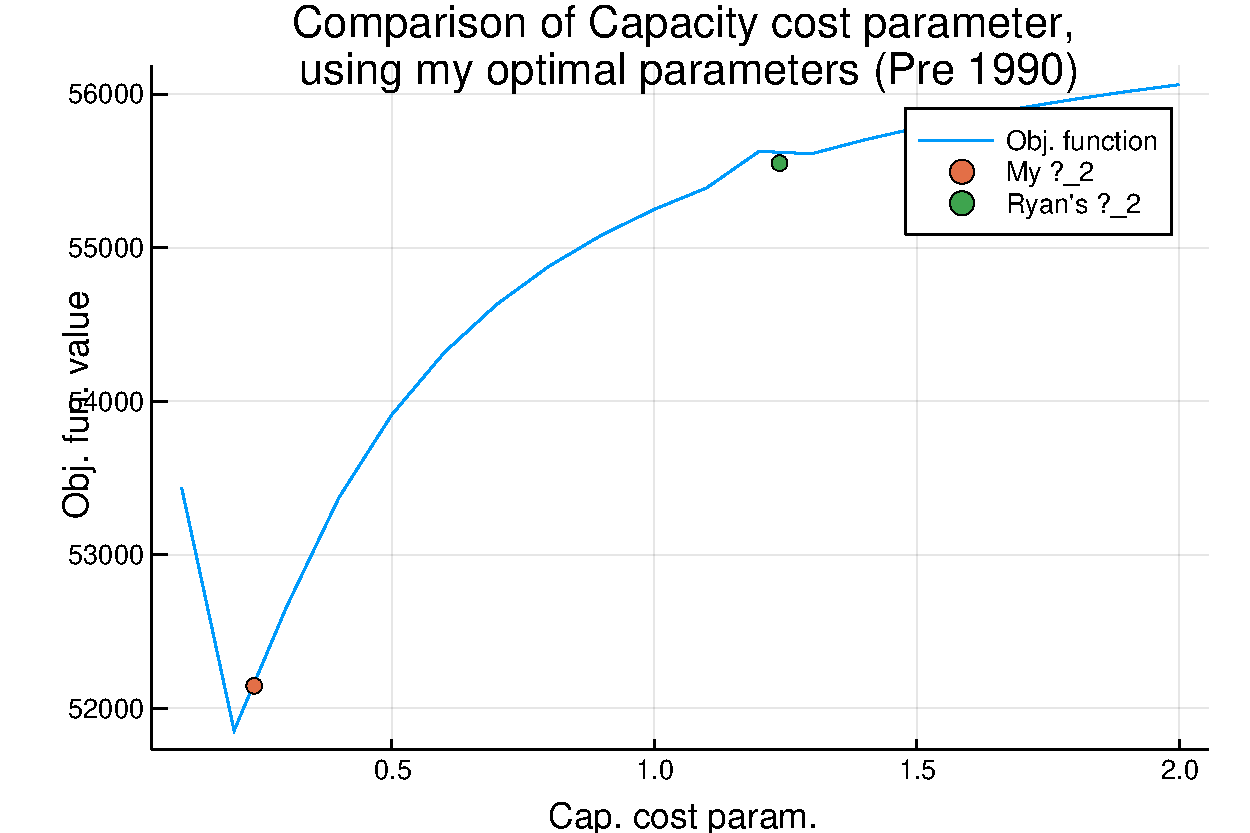
\includegraphics[scale=0.6]{../results/paramcomp-S.pdf} 
\end{center}
\label{fig:d2comp}
\end{figure}

\begin{figure}
\begin{center}
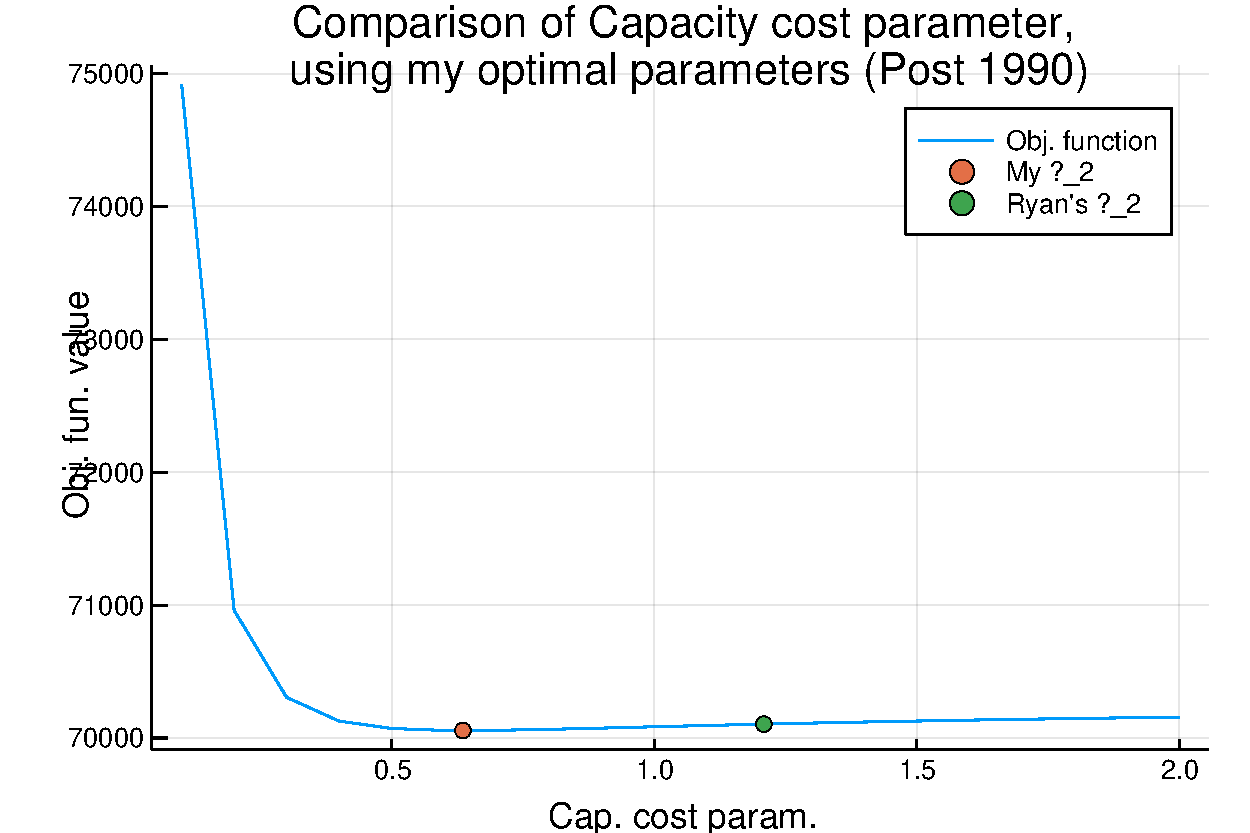
\includegraphics[scale=0.6]{../results/paramcomp-p90-S.pdf} 
\end{center}
\label{fig:d2comp-p90}
\end{figure}

\begin{figure}
\begin{center}
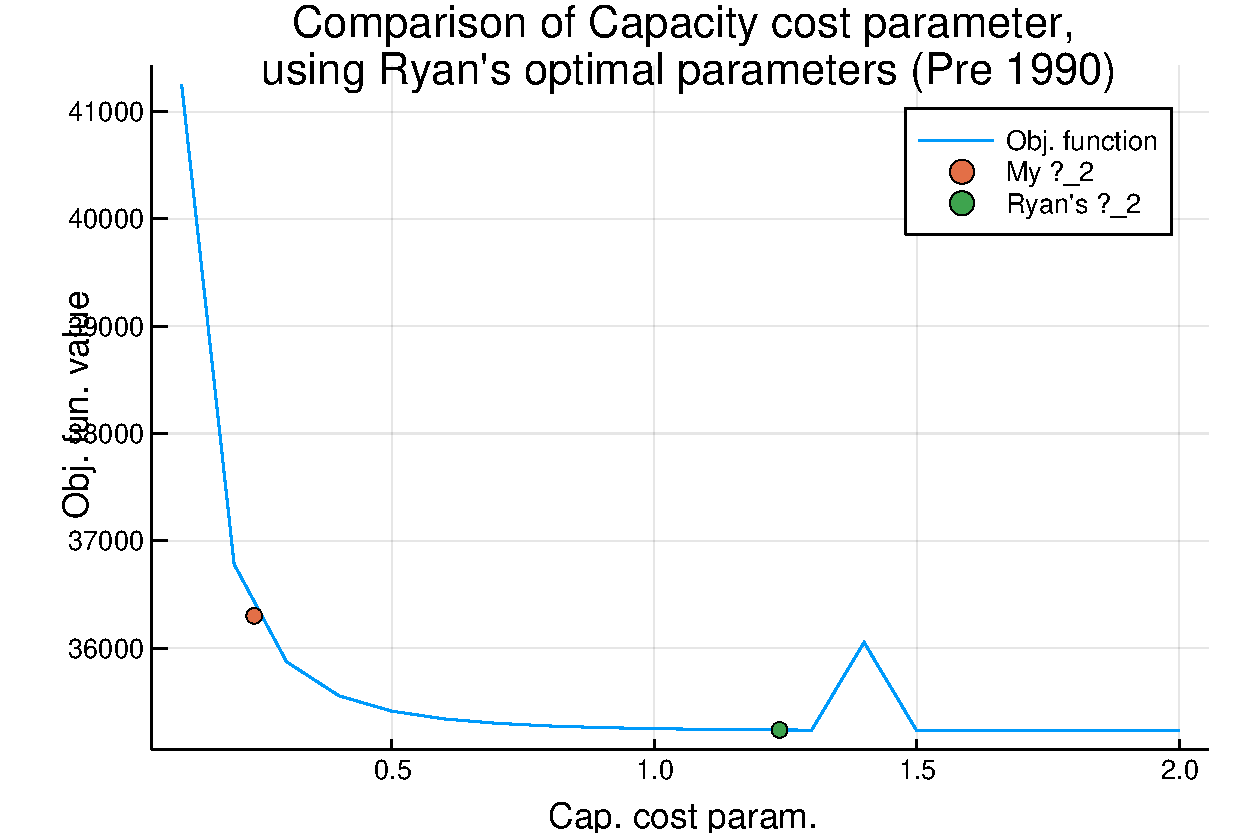
\includegraphics[scale=0.6]{../results/paramcomp-R.pdf} 
\end{center}
\label{fig:d2comp-r}
\end{figure}

\begin{figure}
\begin{center}
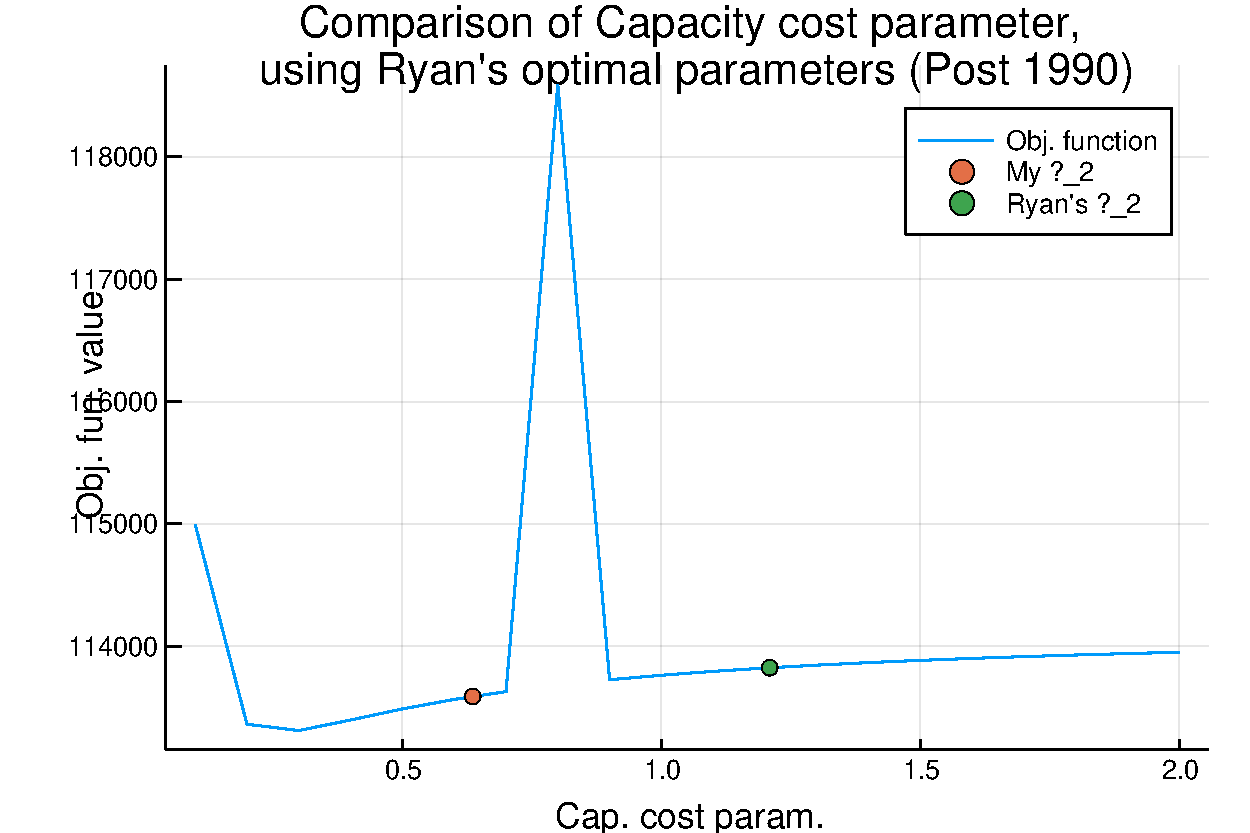
\includegraphics[scale=0.6]{../results/paramcomp-p90-R.pdf} 
\end{center}
\label{fig:d2comp-p90-r}
\end{figure}

\end{document}